%%This is a skeleton file for writing an e-lab paper (University College of Antwerp)
%%Both this file and the accompanying elab.cls file are the worj of Michael Shell (IEEETran)
%%All credit goes to him!


%% Support sites:
%% http://www.michaelshell.org/tex/ieeetran/
%% http://www.ctan.org/tex-archive/macros/latex/contrib/IEEEtran/
%% and
%% http://www.ieee.org/


\documentclass[9pt,journal,compsoc,twoside, a4paper]{elab}



% Some very useful LaTeX packages include:


% *** GRAPHICS RELATED PACKAGES ***
\usepackage[pdftex]{graphicx}
% http://www.ctan.org/tex-archive/macros/latex/required/graphics/
% Another good source of documentation is "Using Imported Graphics in
% LaTeX2e" by Keith Reckdahl which can be found as epslatex.ps or
% epslatex.pdf at: http://www.ctan.org/tex-archive/info/
%
% latex, and pdflatex in dvi mode, support graphics in encapsulated
% postscript (.eps) format. pdflatex in pdf mode supports graphics
% in .pdf, .jpeg, .png and .mps (metapost) formats. Users should ensure
% that all non-photo figures use a vector format (.eps, .pdf, .mps) and
% not a bitmapped formats (.jpeg, .png).

% *** MATH PACKAGES ***
\usepackage[cmex10]{amsmath}
% A popular package from the American Mathematical Society that provides
% many useful and powerful commands for dealing with mathematics.
% http://www.ctan.org/tex-archive/macros/latex/required/amslatex/math/

% *** SPECIALIZED LIST PACKAGES ***
\usepackage{algorithmic}
% algorithmic.sty was written by Peter Williams and Rogerio Brito.
% This package provides an algorithmic environment fo describing algorithms.
% You can use the algorithmic environment in-text or within a figure
% environment to provide for a floating algorithm. Do NOT use the algorithm
% floating environment provided by algorithm.sty (by the same authors) or
% algorithm2e.sty (by Christophe Fiorio) 
% http://www.ctan.org/tex-archive/macros/latex/contrib/algorithms/
% There is also a support site at:
% http://algorithms.berlios.de/index.html

% *** SUBFIGURE PACKAGES ***
\usepackage[tight,normalsize,sf,SF]{subfigure}
% subfigure.sty was written by Steven Douglas Cochran. This package makes it
% easy to put subfigures in your figures. e.g., "Figure 1a and 1b". 
% http://www.ctan.org/tex-archive/obsolete/macros/latex/contrib/subfigure/
% subfigure.sty has been superceeded by subfig.sty.


% *** PDF, URL AND HYPERLINK PACKAGES ***
\usepackage{url}
% url.sty was written by Donald Arseneau. It provides better support for
% handling and breaking URLs. url.sty is already installed on most LaTeX
% systems. The latest version can be obtained at:
% http://www.ctan.org/tex-archive/macros/latex/contrib/misc/
% Read the url.sty source comments for usage information. Basically,
% \url{my_url_here}.


% *** Do not adjust lengths that control margins, column widths, etc. ***
% *** Do not use packages that alter fonts (such as pslatex).         ***

% correct bad hyphenation here
\hyphenation{op-tical net-works semi-conduc-tor}
% Declare graphics path


\begin{document}

% paper title
% can use linebreaks \\ within to get better formatting as desired
\title{WSN localization with the Senseless framework}


\author
{
		Peter~De~Cauwer,
    Tim~Van~Overtveldt,
    Jeroen~Doggen,
    Jerry~Bracke,
    and~Maarten~Weyn.% <-this % stops a space
		\IEEEcompsocitemizethanks
		{
			\IEEEcompsocthanksitem P. De Cauwer, T. Van Overtveldt, J. Doggen, J. Bracke and Maarten Weyn are with the University	College of Antwerp, Paardenmarkt 92, 2000 Antwerp, Belgium\protect\\
			% note need leading \protect in front of \\ to get a newline within \thanks as
			E-mail: see http://www.e-lab.be
		}% <-this % stops a space
		\thanks{Manuscript received June, 2009; revised June 17, 2009.}
}


% The paper headers %Leave like this!
\markboth{Papers of the e-lab master theses' 2008-2009}%
{WSN localization with Senseless framework}

\IEEEcompsoctitleabstractindextext{%
\begin{abstract}
Localization of nodes in wireless sensor networks (WSNs) is important to context-aware and position-dependent applications; data are generally meaningless without a known location. Many algorithms exist for localizing nodes using RSS; however, a detailed quantitative comparison of these algorithms has not yet been published. In this paper, we present such a quantitative comparison of algorithms which use RSS as a ranging method and present a localization software framework called Senseless. We also conducted a survey about the influence of the orientation of a node, thus the radiation pattern. Our study finds that the received power is not equal in all directions and that no single best algorithm for localization exists to date. Each algorithm has a different purpose and diverse properties. Learning from these algorithms and techniques, the correct algorithm can be chosen for the correct environment and a more advanced localization system is feasible. Using this framework, we implemented a coule of centralized algorithms; Multilateration, MinMax, Centroid Localization and Weighted Centroid Localization.
\end{abstract}

\begin{IEEEkeywords}
Wireless Sensor Network, WSN, RSSI, localization, TelosB, TinyOS, Senseless.
\end{IEEEkeywords}
}

% make the title area
\maketitle
\IEEEdisplaynotcompsoctitleabstractindextext

%Leave this part alone, it is pretty fragile!
  \noindent\raisebox{2\baselineskip}[0pt][0pt]%
  {\parbox{\columnwidth}{\section{Introduction}\label{sec:introduction}%
  \global\everypar=\everypar}}%
  \vspace{-1\baselineskip}\vspace{-\parskip}\par

%Now starts your actual paper. Only the first letter of the Introduction needs a larger, so-called
%drop letter. ALL OTHER SECTIONS/SUBSECTIONS START WITH A NORMAL LETTER.

% form to use if the first word consists of a single letter:
% \IEEEPARstart{A}{demo} file is ....
% 
% form to use if you need the single drop letter followed by
% normal text (unknown if ever used by IEEE):
% \IEEEPARstart{A}{}demo file is ....

% You must have at least 2 lines in the paragraph with the drop letter
% (should never be an issue)
% Here we have the typical use of a "W" for an initial drop letter
% and "ireless sensor networks" in caps to complete the first word.
\IEEEPARstart{A}formal definition of Wireless Sensor Networks is given in \cite{akyildiz2002wsn}. The purpose of a WSN is to monitor some physical phenomena such as the ambient temperature, air humidity, and the presence or absence of a certain chemical. Usually, this data is collected at a common point, the data sink, where the data can be further processed or analyzed by the user. WSNs enable a great deal of new applications including environmental and habitat monitoring, smart homes and battlefield control \cite{tolle2005mr} \cite{chong2003sne}.

Accurate and low-cost sensor localization is an essential service and is important to many of these applications. The measured data is generally meaningless without knowing where it originated from. That being said, there are other reasons to acquire the location of a sensor. Location can be a goal in itself, such as in warehousing and manufacturing applications. Another added benefit is the possibility of geographical based routing. 

Given the popularity of GPS, one would think of it as a possible solution. However, this is considered a bad solution because of several reasons. Firstly, a great deal of WSN applications are built  for indoor environments. Clearly, GPS does not suffice as it requires Line-of-Sight with at least four satellites. Secondly, GPS requires significant power to operate, which is a sparse resource in WSNs. Thirdly, GPS adds to the size and cost of a WSN node which should be kept as low as possible. This does not mean, however, that GPS is entirely out of the question. A small number of WSN nodes will need a priori knowledge about their location; this can be done by a GPS receiver or by manually mapping the node to a position on a map, or some other method. The number of these nodes should be kept as low as possible, in order to keep the deployment cost and time low. 

\begin{table}[ht]
\caption{List of abbreviations}
\centering
\begin{tabular}{l l} \hline
	WSN 	& 	Wireless Sensor Network \\
	WSNs  &   Wireless Sensor Networks \\
	RSS 	& 	Received Signal Strength \\
	RSSI  &   Received Signal Strength Indication \\
	TOA   &		Time Of Arrival \\
	AOA   &   Angle Of Arrival \\
	CL 		& 	Centroid Localization \\
	WCL 	& 	Weighted Centroid Localization \\
	ML		&		Maximum Likelihood \\
	LS 		& 	Least Square \\
	LOS   &   Line Of Sight \\
	AN 		& 	Anchor Node \\
	BN 		& 	Blind Node \\
	RN    &   Root Node \\
	GUIs  &   Graphical Unit Interfaces \\ \hline
\end{tabular}
\end{table}

Localization techniques which are specific for WSNs are based on pair-wise measurements between nodes to estimate the positions. A small fraction of the network should have a known position as described in  the previous paragraph. These nodes are called anchor nodes. The other kind of nodes, without a known position, are called blind nodes. Thus, the goal of a localization system is to determine the position of the blind nodes by communicating with the anchor nodes. We can divide these techniques into two categories: range-based and connectivity-based. Range-based methods estimate the distance between nodes with ranging method such as ToA, AoA and RSS. These techniques typically provide superior accuracy but are more complex than connectivity-based  algorithms. These do not estimate the distance between nodes but determine the position of a blind node by their proximity to anchor nodes. \cite{hightower2001lsu}  describe agreement properties of localization techniques in more detail. 
There are other localization techniques which are used in other networks, the most common being RF fingerprinting. In this method, a map based on radio signals is created. In the first phase (offline-phase) we measure RSS on different points on our map and store them in a database. The second phase (real-time phase) measures the RSS of a blind node and compares it to reference points on the map constructed during the first phase, in order to determine the location of the blind node. The problem with this technique is that the RF pattern changes when the environment changes, which means that the radio map is no longer up to date and the accuracy will therefore drop dramatically. A second problem is that these maps are time-consuming to build. Other techniques exist, but they are far less common and unsuitable for WSNs.  These techniques will not be used in this paper. 

Although many ranging techniques exist, in this paper we have narrowed them down to RSS-based ranging. 
RSS-based ranging is founded on the principle that RSS attenuates with distance due to free-space losses and other factors. RSS is generally considered as a bad method because of its high variability due to interference, multipath and shading. Errors can be divided into two categories, environmental and device errors. Environmental errors are due to the wireless channel; these include multipath, shadowing effects and interference from other radio sources. Device errors are generally calibration errors. The most important consideration here is to keep the transmitted power constant, despite inter-device differences and depleting batteries. Environmental errors can also be divided into two parts: rapid time varying errors and static environment dependent errors. The first is due to movement of people, additive noise and interference. This can mostly be modeled as Gaussian noise. As a result, this can be reduced considerably by averaging multiple RSSI measurements. The second type of error is due to the varying properties of the environment, such as multipath and shadowing. Since the layout of the environment and the placement of doors and furniture cannot be known without prior knowledge, this error should be modeled as random. 

In order to create an accurate localization system based on RSS, the wireless channel properties and these other degrading effects must be modeled as accurately as possible. All these factors seem to give RSSI measurements a large random factor, thus making it very unpredictable. Even with very good modeling, it is inevitable that errors remain present because of the random factor; thus any good localization algorithm should also account for these factors. The upside of using RSS as a ranging method is that the radio can be used for communication and localization. This makes RSS very interesting because there is no need for additional hardware. Other ranging methods such as TOA, especially combined with ultrasound, usually yield better results, but require additional specialized hardware which adds to the size and cost of a node.

RSS-based localization can be divided into three categories:
\begin{itemize}
	\item Range-based or fine-grained localization 
	\item Connectivity-based or coarse-grained localization 
	\item RF Fingerprinting, as described in the previous paragraph
\end{itemize}
We will restrict our algorithms to the first two types to satisfy the ad-hoc requirement of the network. 

As WSNs have some unique properties, the algorithms in this paper have been developed or selected with the following goals in mind: 
\begin{itemize}
	\item RSS-based : using this technique no additional hardware is required, thus the cost of a node can be kept low. However, because nodes have an antenna embedded on the PCB, it would be better to have an external antenna as these have a more uniform radiation pattern. 
	\item Distributed and self-organizing: The algorithm should be able to run locally on the nodes to avoid a central processing dependency. This is especially important for WSNs due to the fact that individual nodes and links between nodes are more prone to failure than in a traditional computing environment. Batteries may be depleted and radio links can be obscured.  
	\item Robust: The algorithms should account for localization errors and node failures. 
	\item Receiver-based: The task of localization is up to the blind node so that the network scales well. 
	\item Responsiveness: The localization latency needs to be kept as low as possible. Mobility is fairly limited in WSNs as most nodes have a static position; however, certain nodes can be mobile, so this factor needs to be accounted for as well. 
	\item Energy usage: Given the sparse amount available, processing and communication needs to limited. Unfortunately, this means that certain applications are not suitable for WSNs because of the high computational requirements and the lightweight microcontroller that drives the nodes. Communication between nodes needs to be limited as well because the radio requires much more power than the microcontroller. 
	\item Adaptive: We want our algorithm to be adaptive to the number of ANs and the density of the network. If the density or the number of ANs rises, the accuracy should improve. The algorithm should thus benefit from the high density of the WSN. The algorithm should still perform well with a low network density and AN ratio. 
	\item Multihop localization: Nodes not in range of an AN should still be able to localize themselves by the use of other BNs, this is referred to as cooperative or multihop localization \cite{patwari2005lnc}, compared to single-hop localization, where only blind nodes in range of enough anchor nodes can determine their position. 
\end{itemize}

The main contributions of this paper are: 
\begin{itemize}
	\item We present an overview of the existing algorithms and literature. 
	\item We compare three algorithms with quantitative measurements. 
	\item We researched the influence of the orientation of a node compared to a node with an external antenna.
	\item We present Senseless, a software framework to manage WSN localization.
	\item We interface this framework to Scala, a localization middleware project. 
\end{itemize}

The rest of the paper will be organized as follows: chapter two summarizes related work, and provides an overview of the suitable algorithms and work that contribute to building a good algorithm; chapter three presents our software framework; chapter four presents the ranging and the various algorithms that we have implemented and tested framework; in chapter five the methods and results are presented and we conclude in chapter six. 
\section{Related Work}
The amount of literature on this topic is quite substantial. It becomes more manageable if we limit ourselves to three categories: ranging algorithms, location estimation and frameworks. Limited surveys on this topic do exist; however, they fail to point out a superior algorithm and provide few quantitative comparisons, so further investigation is required. 

Sum Dist is a distributed multihop algorithm that makes use of the hop count as a primitive distance metric \cite{langendoen2003dlw}. The distance to the anchor nodes is determined by simply adding the ranges (RSS) encountered at each hop during the network flood of beacon messages by the anchor nodes. The downside of this algorithm is that the range errors rise exponentially when the beacon message travels over multiple hops. Thus, in large networks with little anchor nodes, it will lead to poor ranging. A good alternative is DV-hop. It makes use of the topological information; counting the hops instead. When the topology of the network is very irregular, the ranging will be very inaccurate because of the high variance in hop distance. The anchor nodes broadcast a beacon message to the blind node, which will forward the message to the blind nodes that are out or range of the anchor nodes after filling in the hop count as the path length.
The paper "RSS-based location estimation with unknow pathloss model" \cite{li2006rbl} dynamically estimates the distance-power gradient; parameter of the radio propagation pathloss model \cite{seidel1992mpl}. It adapts automatically to the environment, thus eliminating the need for extensive channel measurements. This  leads to a more accurate conversion of RSS to distance.
Sorted RSSI Quantization \cite{li2005srq} is a connectivity based algorithm that uses hopcount and RSS as a ranging method. It multiplies a hop by the radio range or a chosen distance. It sorts the obtained RSSI and applies a quantizer that represents a level of range in the hop. This makes the algorithm insensitive to RSSI errors.

MoteTrack\cite{lorincz2007mrd} is decentralized location tracking system based on RF. It is similar to RADAR \cite{bahl2000rbr}, but does not rely upon back-end server or network infrastructure. The location of each blind node is computed using a RSS signature from the anchor nodes to a database of signatures. This database is stored at the anchor nodes themselves.
Cricket \cite{priyantha2000cls} is decentralized and uses RF and ultrasound to determine the location of a blind node. Anchor nodes broadcast beacon messages, together with te RF message, it will transmit a ultrasonic pulse. Blind nodes listen to beacon messages and upon receipt, they will listen to the corresponding ultrasonic pulse. A distance to the transmitting anchor node can be estimated with that pulse.
A noteworthy survey is \cite{langendoen2003dlw} by K. Langendoen. This survey describes three algorithms: 
\begin{itemize}
	\item Ad-hoc positioning by Niculescuand Nath \cite{niculescu2003dbp}, 
	\item N-hop multilateration by Savvides et al. \cite{savvides2003nhm}, 
	\item Robust positioning by Savarese et al. \cite{savarese2002rpa}. 
\end{itemize}
These algorithms are fully distributed algorithms; they require no central processing node and are designed towards multihop localization. The survey concludes that no single algorithm performs best under different circumstances. Robust positioning works best when no or very bad ranging information is available. Ad-Hoc positioning only works well when the ranging error is very low ((<)20\%). The N-hop multilateration is to be preferred in other situations. 

This survey identifies a common three-phase structure in these localization algorithms. The first phase determines the distances between blind and anchor nodes. Note, however, that this does not mean that a specific ranging method, such as RSS, should be used,. The second phase derives a position using the RSS from the anchor nodes. These two phases are roughly equal to what was described in the introduction. Finally, there is a third phase called the refinement phase, where the positions are refined through iterative measurements. 

Another comparison is given in \cite{zanca2008ecr} by Zanca et.al. This paper compares four algorithms: 
\begin{itemize}
	\item Min-Max \cite{langendoen2003dlw}\cite{nguyen2003las}
	\item Multilateration \cite{langendoen2003dlw}\cite{nguyen2003las}
	\item Maximum Likelihood \cite{patwari2001rlw} by Patwari N.
	\item ROCRSSI \cite{liu2004slr} by Liu C.
\end{itemize}
A brief introduction to the radio channel is provided. The absolute ranging errors of the algorithms are presented with the number of anchor nodes as a parameter. The authors conclude that ML provides superior accuracy compared to the other algorithms when the number of anchor nodes is high enough. Interestingly, despite its simplicity, Min-Max achieves reasonable performance. This is probably due to the fact that it localizes the node in the center of the estimated area. The authors also note that a good radio channel model is required to obtain a relatively high accuracy. The algorithms presented in this paper are one-hop algorithms; they can only localize nodes in reach of enough anchor nodes.
\section{Framework}
We have developed a software framework, Senseless, which provides a common data interface to the WSNs and GUIs. It also controls the data flows between the WSNs and GUIs, and stores this data in a database for later retrieval. The system is capable of working with different algorithms and new algorithms can be easeliy added. If there are three anchor nodes available, we can work with range-based algorithms, thus obtaining a better accuracy. If, on the other hand, only one anchor node is available, a connectivity-based algorithm can and must be used. We will use this system to test the different localization algorithms and analyze the RSS data. 

Senseless has a Model-View-Controller (MVC) design, as in Figure \ref{fig:mvc}; the system is divided into three different parts each with different tasks. The separation of these responsibilities enhances the modularity of the system. 
The details of this design are as follows:
\begin{itemize}
	\item Model: This layer defines the representation of the information which the application works with. The data is stored in a MySQL database. 
	\item View: Information can be accessed and controlled via this part. User interfaces are defined in this layer. The view does not process data. 
	\item Controller: It processes and uses polling to react to events, mostly caused by the actions of the user and the data delivered by the WSN. 
\end{itemize}
The advantage of this design pattern is that we can easily add views and models without changing the whole system. 

\begin{figure}[h]
	\centering
		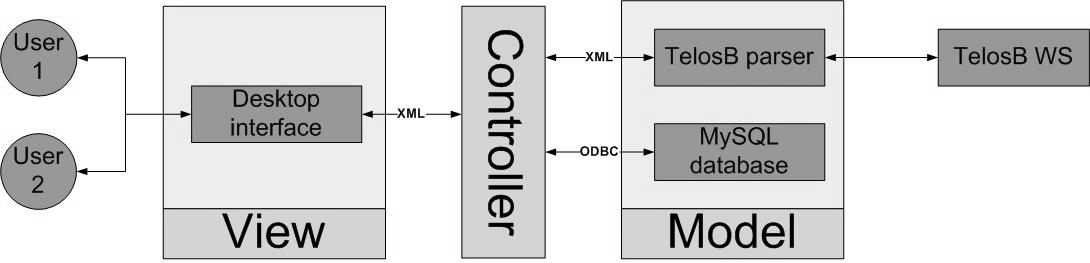
\includegraphics[scale=0.30]{Images/mvc.jpg}
	\caption{The Model-View-Controller design}
	\label{fig:mvc}
\end{figure}

\subsection{Functionality}
The system consists of four main parts:
\begin{itemize}
	\item WSN
	\item Database
	\item Graphical Unit Interface (GUI)
	\item Controller
\end{itemize}

\subsubsection{WSN}
The WSN consists of Telos rev.B nodes, which have the following specifications: 
\begin{itemize}
	\item TI MSP430 microcontroller with 10kB RAM 
	\item IEEE 802.15.4 compliant CC2420 radio: it supports eight discrete power levels and 16 channels
	\item Integrated temperature, light, humidity and voltage sensor 
	\item TinyOS 2.X compatible 
	\item Programmable via USB interface 
	\item Integrated antenna 
\end{itemize}

Each node fulfills one of the three different roles: 
\begin{itemize}
	\item Root node (RN): this node receives data from the rest of the network , and acts as a bridge between the WSN and the rest of the framework. The root sends these messages to the controller via an XML parser. It also receives commands from the controller and disseminates these to the right node.
	\item Anchor node (AN): this node has a known location, and broadcasts a message with its ID to the blind nodes and anchor nodes for calibration. The node also transmits its sensor data to the root with the sensor message. 
	\item Blind node (BN): this node has an unknown location and receives broadcast messages from the anchor nodes. The node uses these messages to determine the RSS, and transmits the RSS together with the ID of the anchor node to the root with the location message. The blind node also transmits its sensor data to the root node with the sensor message. 
\end{itemize}

There are three different data messages which are collected from the wireless network:
\begin{itemize}
	\item	Sensor messages, which contain the data collected by the sensors of the nodes.
	\item Location messages, which contain data relevant to locate the blind node.
	\item Status messages, which contain data that represent the status of the node transmitting the message.
\end{itemize}

\subsubsection{Database}
We implemented a MySQL 5.0 database to store the data generated by the system, but any ODBC-compliant database can be used.  

\subsubsection{GUI}
The user interfaces provides us with the ability to easily control and monitor the WSN. Rapid deployment was the key motivator to build this component. Using this, the user can set several node parameters, with a focus on localization: sampling period, coordinates (in meters), inactive/active, blind/anchor and the leds. This can be done in a few seconds. In contrast to manually hardcoding every single node of the network, which can be very time-consuming and sometimes impossible due to the fact that TinyOS-programmed nodes and other types of nodes usually provide very little to no user interaction. 

\subsubsection{Controller}
The controller is the core of our system. The controller is programmed in C# using the .NET 3.5 framework.  It is divided into several class library's and a single Windows Forms project.

It has four main functions:

Firstly, the controller acts as a gatekeeper to the database, ensuring that all data is stored in the correct table and is of the correct type. This is especially important for WSNs as a plethora of hardware platforms exist. These platforms have different data types and can have a different endianness.

Secondly, the controller is also a central gathering point for all the data. By using the controller in our framework, every other component can use a single data interface and should only be aware of the location of the controller.

Thirdly, an interface to Scala is provided as well. Scala is a middleware for location systems. Scala and the interface will be described in the designated section.
Finally, the controller implements the centralized versions of our localization algorithms. The user can instruct the controller to use an algorithm via a simple Windows Forms GUI.

\textbf{WSN vs Controller}

The communication between the WSN and the controller is done with an XML parser, which translates the messages of both sides into XML and back into an internal format. The root node of the WSN receives all the messages (sensor, location and status) from the nodes and forwards these to the controller, or if the controller needs to pass a command on to the root, it will be forwarded to the root. With the help of the dissemination protocol, the command is transmitted over the WSN. 

\textbf{Controller vs GUI}

The communication between the controller and the GUI also happens with an XML parser, which translates the messages that need to be exchanged. Firstly, the GUI displays the data from the WSN, thus a request needs to be send to the controller. The controller receives the request, and gets the data out of the database and sends it to the GUI. Secondly, the GUI is used to control the WSN. If, for example, you want to change the sample rate of the WSN, then a command will be sent to the controller which forwards it to the root node of the WSN. 

\textbf{Controller vs Database}

The communication here makes use of ODBC (Open Database Connectivity), which is an universal database interface. By using this interface, the controller does not need to worry about the database that is used. Stored procedures are used instead of full SQL syntax.

\subsection{SCALA}
Scala is a TETRA \cite{tetra} project which aims to shorten the gap between localization technologies and possible end-user applications. The goal of this project is to ease the development of location aware applications by providing these applications with a common interface to the location technologies.

From a technical point of view, Scala adapts the interfaces of the existing localization technologies into a common interface. Doing so, the user can receive location information transparent of the underlying technology. 
Another feature of Scala is the fusion of location information. By combining the information the middleware receives from different localization technologies, a more accurate and robust position can be determined.

The Senseless framework provides an interface to SCALA. The framework will plug into SCALA as an engine. Doing so, our algorithms become accessible to a variety of applications.
The interface with Scala is performed in the controller via WCF \cite{WCF}. Currently our engine supports four distinct software interfaces. 

\begin{\begin{itemize}
	\item Map data
	\item Position data
	\item Context data, such as the data coming from the sensors
	\item Availaible nodes
\end{itemize}}

Two types of communication are available: polling and event-based. By polling the engine, information is requested only when needed, as opposed to event-based communication where, Scala subscribes to information coming from the framework. The interface is loosely based on the ANSI Rtls API \cite{RTLS}.
The API documents a polling-based system. Possible data fields are specified and a method of filtering data is documented as well.

\section{Localization}
Localizing the position of a node happens in 2 phases:
the first phase is the ranging: the estimation of the distance from an anchor node to the blind node. This is done with a propagation model: translates the RSSI to distance. This model can be made more accurate if you apply a calibration process.
The second phase is calculating the node with an algorithm.

\subsection{Propagation model}
There exist a number of propagation models:
\begin{itemize}
	\item the Rayleigh fading model\cite{hashemi1993irp}: does not account for a Line Of Sight (LOS) component
	\item Rician distribution model\cite{rice1944mar}: the determination of the model parameters is difficult
	\item Floor attenuation factor propagation model\cite{seidel1992mpl}: manual determination of model parameters
	\item log-normal-shadowing model\cite{seidel1992mpl}: the most simpel model
\end{itemize}
We use the log-normal-shadowing model for the ranging. It is the most widely used signal propagation model and the determination of the parameters is simple and can be obtained dynamically with Least Squares (LS).
\[
RSS(d) = PT - PL(d0) - 10\times n \times \log( \frac{d}{d0} )+ Xo
\]
Where, \textsl{PT}	is the tramitted power, \textsl{PL(d0)} is the path loss for the reference distance \textsl{d0}, \textsl{n} is the path loss exponent (the rate at which the path loss increases with distance) and \textsl{Xo} is a gaussian random variable with zero mean and standard deviation \textsl{o} dB.
The most common reference distance is one meter. In the calibration phase of the WSN, we determine the path loss exponent and the path loss for the reference distance, so that the propagation model is adapted to the environment and thus more accurate.

\subsection{Algorithms}
Centroid localization is a simple approach for coarse grained localization. All blind nodes calculate their position as the centroid of the anchor nodes within their communication range. This algorithm has a low accuracy because it does not use signal strength to denote the range. A solutions to make CL more accurate is the Weighted Centroid Localization (WCL)\cite{schuhmann2008iwc}. A weight is coupled to each anchor by its RSSI:
\[
Weight = \frac{1}{RSS^{g}}
\]
The degree \textsl{g} has to ensure that the remote anchor nodes still have impact on the position determination. In case of a very high \textsl{g}, the calculated position
moves to the closest position of the anchor node and the positioning error increases.

Min-Max is a popular and a very easy algorithm to implement. Anchor nodes, that are in range of the blind nodes, will create a box around them. This box has the anchor node as the center and has a height and width of twice the estimated distance to the blind node. In an ideal situation, will this algorithms work, but the estimated distance between the node is often underrated. So, one or more boxes will not collide and thus a location can not be determined. In this case, the estimated distance between the nodes is expanded with 10\% until all boxes collide.

Multilateration is used in a variety of localization systems including GPS. Multilateration calculates the intersection of three or more circles. If these circles intersect in exactly one point, the coordinates of this point can be determined by linear equations.  This method has one major flaw; the circles almost never intersect in a single point. They do not intersect at all or overlap a part of each other. In more dramatic cases one circle can entirely overlap another circle.  This is due to the erroneous ranging. The range is over or underestimated. 

\cite{trilat} presents two solutions to solve this problem. The first solution is based on non-linear LS . Through an iterative process the range of the circles is changed until a single point of intersection is found. This method can yield fairly accurate results. The downside however is that it is computationally intensive. The second solution is much simpler and requires that the circles overlap. Given x circles, the algorithm determines the x-nearest points. The centroid of these points is taken as the result. 
The second solution is simpler to implement but has the requirement that the three circles should overlap a part of each other. We present a simple solution to this problem. There are three cases in which the range of the circle should be modified:
\begin{itemize}
	\item The circles are too far from each other and do not intersect 
	\item One circle completely overlaps another circle
	\item A circle is completely inside another circle
\end{itemize}
In each of these cases the range should be adapted accordingly until these conditions are no longer met. The algorithm iterates through all the circles so that all circles are slightly changed instead of drastically changing one circle. The algorithm finally converges to the situation where all circles overlap each other.
We chose to implement both, but an easier from of the first solution namely the normal least square\cite{sayed2005nbw}, this algorithm is much simpler to implement and has a better performance.

\section{Method}
\subsection{Test environment}
Our experiments were performed in an indoor an outdoor environment. The indoor tests were done in a living room which houses a considerable amount of electronics including Wifi equipment operating in the same frequency range. People were walking in the room as well to further interfere with the signal. The outdoor test were done on a local basketball court. Nodes were placed at about five to ten meters from the fencing and few people were walking by.

\subsection{Antenna orientation}
The relative antenna orientation between receiver-transmitter pairs is a major factor in signal strength variability, even in the absence of multipath and shading effects\cite{lymberopoulos2006ecr}. This is due to the fact that antenna's are not perfectly omnidirectional. Ideally, the radiation pattern of an antenna should be uniform and it should look like a circle (2-D space) or a sphere (3-D space). However, in practice, the orientation of the antenna can influence the signal strength by several decibels. Thus, different antenna orientations can produce different sets of RSS values for the same distances between receiver and transmitter, increasing the position error.

Therefore, it is imperative that the antenna's orientation should be accounted for as well. One possible solution would to use a compass to determine the nodes orientation. Given the antennas radiation pattern the transmitted power can easily be obtained. 

A straightforward solution would be to use a more omnidirectional antenna to minimize these effects. For example, Telos rev.B nodes use an onboard antenna. The power received from this antenna can differ by as much as 20dB depending on the orientation.  Fortunately, an external antenna is supported. This can be mounted on the circuit board via an optional standard SMA connector. 

We tested the difference between a node employed with and without an external antenna.

\subsubsection{Set up}
Two Telos rev. B nodes were set in the outdoor environment. 
The test exists out of two parts:
In the first part, the two nodes are equipped with an external antenna with a gain of 6dBi and placed at a distance of one meter and at a distance of five meters from each other at a height of one meter. This way the ground will attenuate the signal. One node is set as an anchor node and will broadcast beacon messages at a rate of 200 ms. The anchor node was rotated and samples were taken at every 20 degrees. The other node, the blind node sends the RSS readings to the database. Approximately 25 samples were collected at every orientation.

In the second part, only one node is equipped with the external antenna and placed at a distance of one and five meter. This node is set as the blind node and receives ideally the same power in every direction. The other node with an integrated antenna is the anchor node that will broadcast the beacon messages. 

\subsection{In \& outdoor positioning}
The following experiment was devised to test the accuracy of our developed localization algorithms.

\subsubsection{Set up}
We placed a total of 10 nodes in both the indoor and outdoor environment. Nine of them are configured as anchor nodes and the last one if configured as a blind node. Every node is placed at a height of one meter.
The anchor nodes are placed randomly at fixed locations (in meters):
\begin{itemize}
	\item Node one: 1.19  ; 6.98
	\item Node two: 2.00 ; 8.48
	\item Node three: 3.00 ; 1.50
	\item Node four: 3.19 ; 6.23
	\item Node five: 1.19 ; 5.14
	\item Node six: 4.64 ; 3.88
	\item Node seven: 4.67 ; 0.00
	\item Node eight: 2.50 ; 0.00
	\item Node nine: 0.00 ; 0.00
\end{itemize}
The blind node will be located at the following locations (in meters):
\begin{enumerate}
	\item 5.07 ; 8. 48
	\item 5.07; 4.63
	\item 2.00 ; 1.50
	\item 0.00 ; 3.29
	\item 3.19 , 6.23
	\item 1.19 , 8.48
\end{enumerate}



\section{Results}
\subsection{Antenna orientation}

\begin{figure}[h]
	\centering
		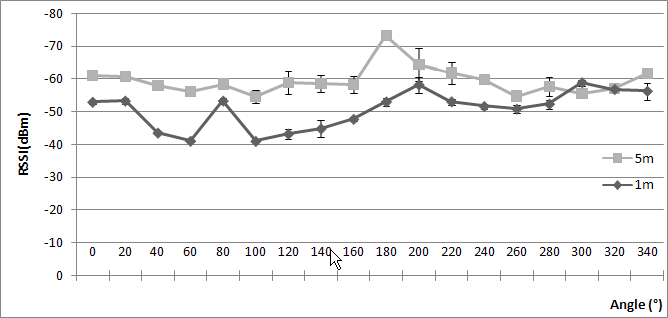
\includegraphics[scale=0.35]{Images/OnboardAntenna.png}
	\caption{Average RSSI at a distance of 1m and 5m with one node equiped with an external antenna}
	\label{fig:OnboardAntenna}
\end{figure}

\begin{figure}[h]
	\centering
		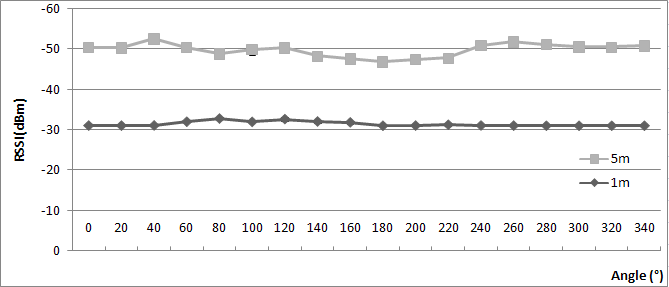
\includegraphics[scale=0.35]{Images/ExternalAntenna.png}
	\caption{Average RSSI at a distance of 1m and 5m with the two nodes equiped with an external antenna}
	\label{fig:ExternalAntenna}
\end{figure}

\begin{table}[ht]
\caption{Table with average RSSI and standard deviation}
\label{table:resultsorient}
\centering
\begin{tabular}{|l|l|l|l|} \hline
\multicolumn{4}{|c|}{Results} \\ \hline
\multirow{} & Average & Stdv1 & Stdv2 \\ \hline
\multirow{Onboard antenna at one meter} & -50,65 & 1,144 & 5,71 \\ \hline
\multirow{Onboard antenna at five meter} & -59,50 & 1,63 & 4,31 \\ \hline
\multirow{External antenna at one meter} & -31,46 & 0,21 & 0,64 \\ \hline
\multirow{External antenna at five meter} & -49,77 & 0,90 & 1,61 \\ \hline
\end{tabular}
\end{table}

Figure \ref{fig:OnboardAntenna} and \ref{fig:ExternalAntenna} display the mean and standard deviation of the RSS when rotating the node. Table \ref{table:resultsorient} displays the average standard deviation for each orientation and the standard deviation of the entire dataset. Note that the standard deviation is sometimes too small to be seen on the graph. These results show that RSS readings are more stable when the node is equipped with a more omnidirectional antenna. However the readings with onboard antenna are fairly stable as well. The results also clearly show that the external antenna is more invariant to orientation than the onboard antenna. 
The results are consistent with the common belief that node orientation influences RSS readings.

\subsection{In \& outdoor positioning}
Figure \ref{fig:IndoorAccuracy} and \ref{fig:OutdoorAccuracy} show the relative positioning error for respectively the indoor and outdoor positioning. The relative positioning error is measured as the absolute positioning error divided by the average distance to every connected anchor node.


The relative positioning error of the algorithms in the outdoor environment is generally below 140\%. The two trilateration algorithms perform really poor in the indoor environment. While Min-Max has a maximun relative positioning error of 68\% and keeps dropping when more anchors are added.
\begin{figure}[h]
	\centering
		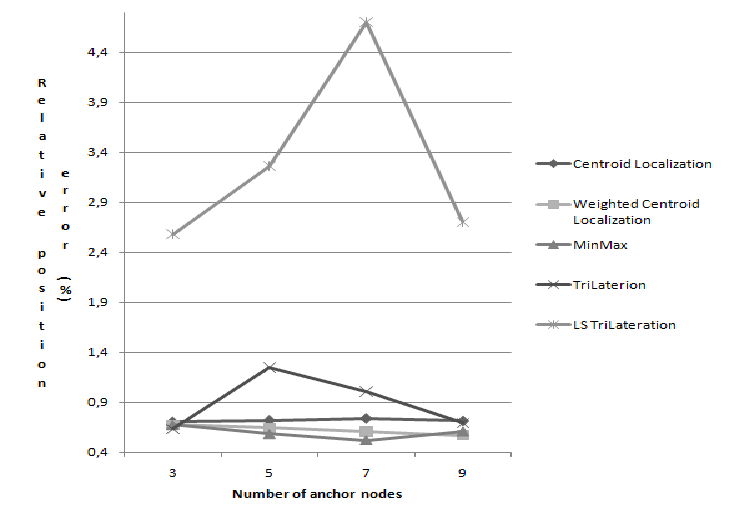
\includegraphics[scale=0.5]{Images/IndoorAccuracy.png}
	\caption{Average relative positioning error in the indoor environment}
	\label{fig:IndoorAccuracy}
\end{figure}

The relative positioning error of the algorithms in the outdoor environment is generally below 80\%. The trilateration with least squares has good computational performance but a very low accuracy in most cases. A better solution would be to use a more advanced form of least square like the weighted least square and the non-linear least square.
Min-Max has the best accuracy, even under 50\%.
\begin{figure}[h]
	\centering
		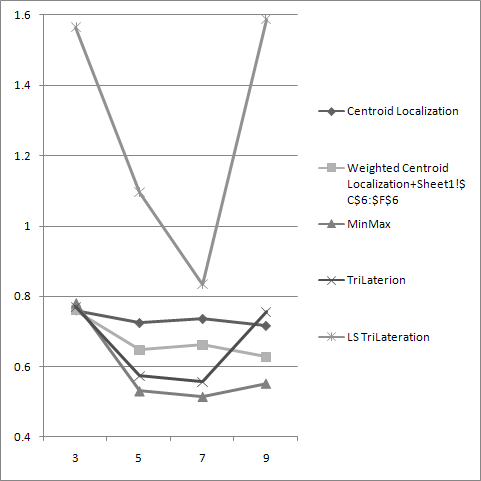
\includegraphics[scale=0.5]{Images/OutdoorAccuracy.png}
	\caption{Average relative positioning error in the outdoor environment}
	\label{fig:OutdoorAccuracy}
\end{figure}
The results show that the accuracy improves when more anchor nodes are added to the system, but we do notice that the accuracy becomes stagnated when we reach the number of 7 anchor nodes. The trilateration algorithms lags behind in accuracy compared to the other algorithms. The Min-Max algorithm is computationally simple and devilers the best accuracy. Therefore it is our current algorithm of choice.
\section{Conclusion}
This paper has investigated the core aspects of WSN localization systems using RSS. Different types of localization systems were introduced and important properties were discussed as well. An overview of our localization framework was given. Three centralized localization systems were discussed.

% references section

% can use a bibliography generated by BibTeX as a .bbl file
% BibTeX documentation can be easily obtained at:
% http://www.ctan.org/tex-archive/biblio/bibtex/contrib/doc/
% The IEEEtran BibTeX style support page is at:
% http://www.michaelshell.org/tex/ieeetran/bibtex/
\bibliographystyle{IEEEtran}
% argument is your BibTeX string definitions and bibliography database(s)
\bibliography{IEEEabrv,bibliografie}



% biography section
% This biography should contain firsylt your formal introduction (e.g. previous work, education, degrees, etc) but should also contain some more 
%personal information (should you wish) such as sports, hobbies, etc. (try to keep this professional though).
\begin{IEEEbiography}[{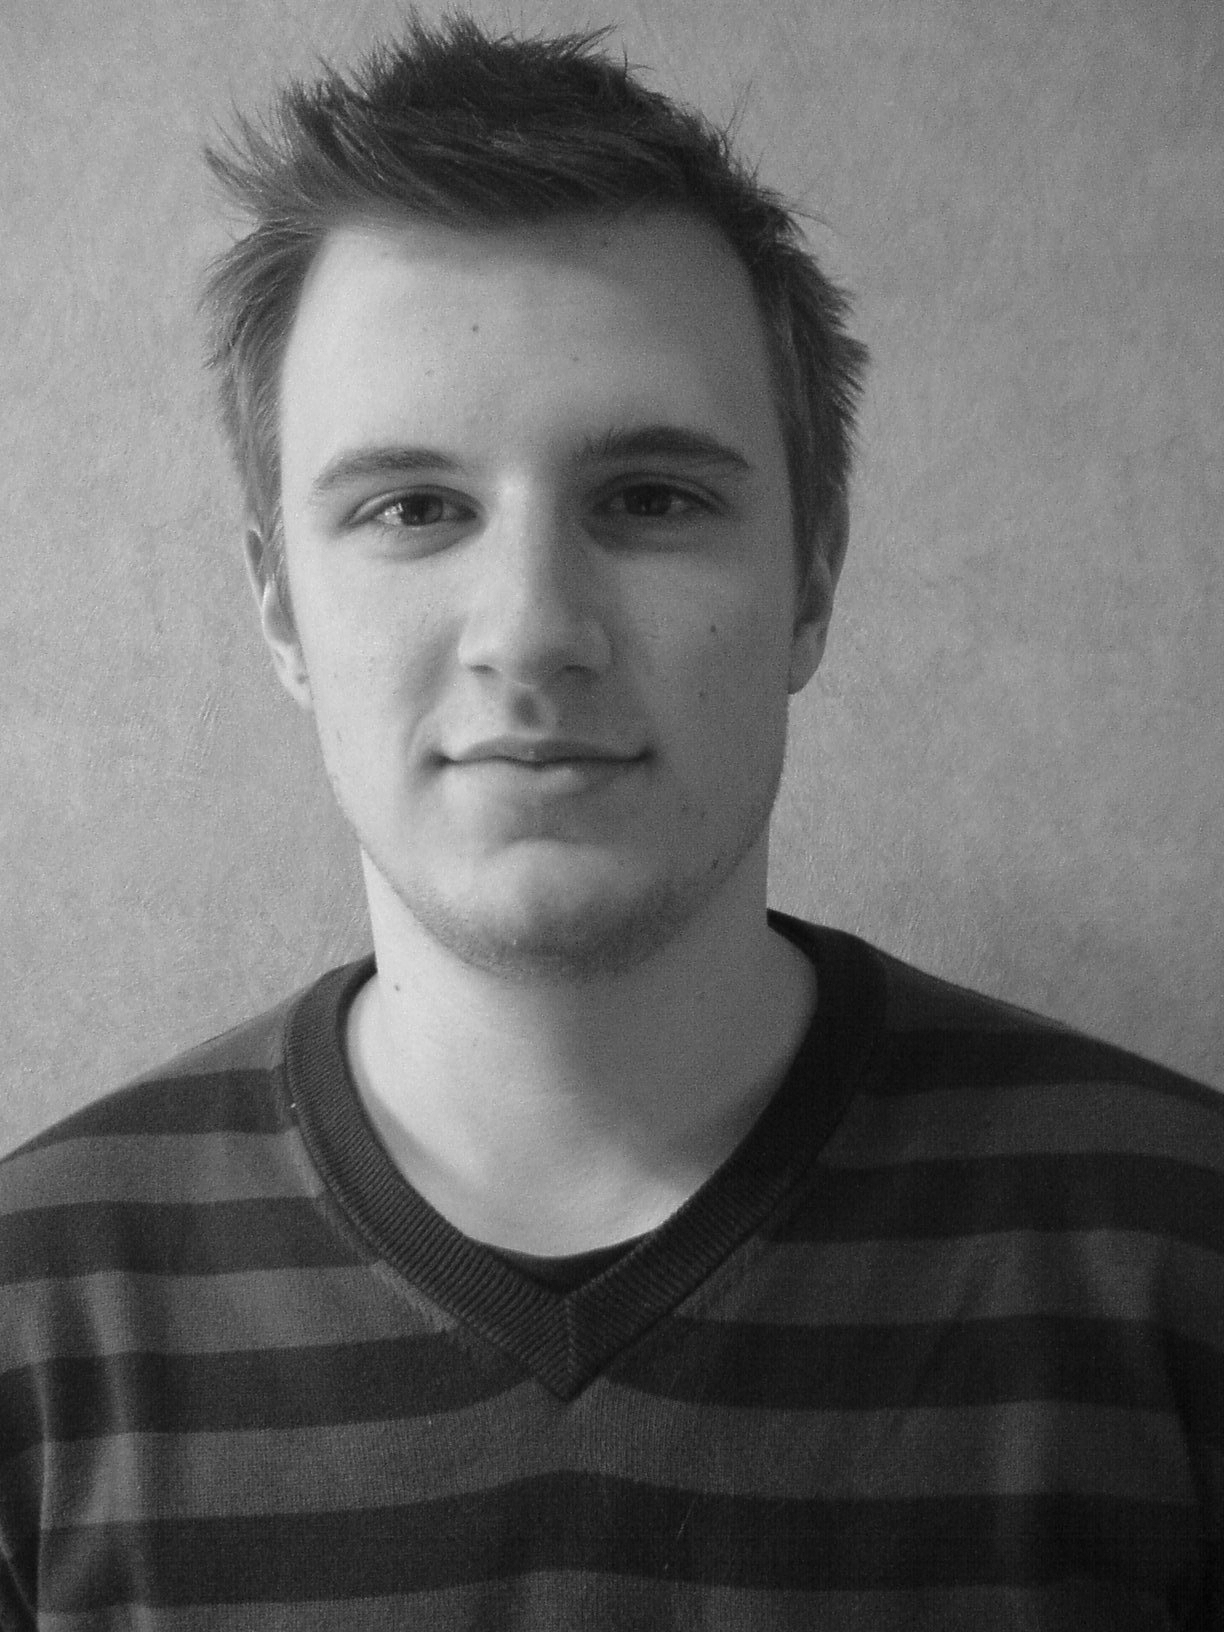
\includegraphics[width=1in,height=1.25in,clip,keepaspectratio]{Images/peter.jpg}}]{Student 1}
Peter De Cauwer is currently working
on his Master Thesis after graduating as
Bachelor in Applied Engineering: electronics-ict
in 2008 at the University College of Antwerp.
\end{IEEEbiography}
\begin{IEEEbiography}[{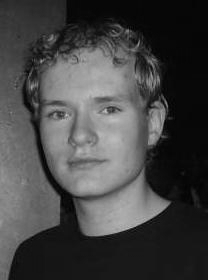
\includegraphics[width=1in,height=1.25in,clip,keepaspectratio]{Images/tim.jpg}}]{Student 2}
Peter De Cauwer is currently working
on his Master Thesis after graduating as
Bachelor in Applied Engineering: electronics-ict
in 2008 at the University College of Antwerp.
\end{IEEEbiography}

If you wish to cite this paper, please use the following code:
Peter De Cauwer, Tim Van Overtveldt, Jeroen Doggen, Jerry Bracke and Maarten Weyn, WSN localization with Senseless framework, Master's Thesis,Department of Apploed Engineering, University College of Antwerp, Belgium, June 2009
\vfill

% that's all folks
\end{document}


